% Options for packages loaded elsewhere
\PassOptionsToPackage{unicode}{hyperref}
\PassOptionsToPackage{hyphens}{url}
%
\documentclass[
]{article}
\usepackage{amsmath,amssymb}
\usepackage{lmodern}
\usepackage{ifxetex,ifluatex}
\ifnum 0\ifxetex 1\fi\ifluatex 1\fi=0 % if pdftex
  \usepackage[T1]{fontenc}
  \usepackage[utf8]{inputenc}
  \usepackage{textcomp} % provide euro and other symbols
\else % if luatex or xetex
  \usepackage{unicode-math}
  \defaultfontfeatures{Scale=MatchLowercase}
  \defaultfontfeatures[\rmfamily]{Ligatures=TeX,Scale=1}
\fi
% Use upquote if available, for straight quotes in verbatim environments
\IfFileExists{upquote.sty}{\usepackage{upquote}}{}
\IfFileExists{microtype.sty}{% use microtype if available
  \usepackage[]{microtype}
  \UseMicrotypeSet[protrusion]{basicmath} % disable protrusion for tt fonts
}{}
\makeatletter
\@ifundefined{KOMAClassName}{% if non-KOMA class
  \IfFileExists{parskip.sty}{%
    \usepackage{parskip}
  }{% else
    \setlength{\parindent}{0pt}
    \setlength{\parskip}{6pt plus 2pt minus 1pt}}
}{% if KOMA class
  \KOMAoptions{parskip=half}}
\makeatother
\usepackage{xcolor}
\IfFileExists{xurl.sty}{\usepackage{xurl}}{} % add URL line breaks if available
\IfFileExists{bookmark.sty}{\usepackage{bookmark}}{\usepackage{hyperref}}
\hypersetup{
  pdftitle={EDA for NBA},
  pdfauthor={Austin Stephen},
  hidelinks,
  pdfcreator={LaTeX via pandoc}}
\urlstyle{same} % disable monospaced font for URLs
\usepackage[margin=1in]{geometry}
\usepackage{graphicx}
\makeatletter
\def\maxwidth{\ifdim\Gin@nat@width>\linewidth\linewidth\else\Gin@nat@width\fi}
\def\maxheight{\ifdim\Gin@nat@height>\textheight\textheight\else\Gin@nat@height\fi}
\makeatother
% Scale images if necessary, so that they will not overflow the page
% margins by default, and it is still possible to overwrite the defaults
% using explicit options in \includegraphics[width, height, ...]{}
\setkeys{Gin}{width=\maxwidth,height=\maxheight,keepaspectratio}
% Set default figure placement to htbp
\makeatletter
\def\fps@figure{htbp}
\makeatother
\setlength{\emergencystretch}{3em} % prevent overfull lines
\providecommand{\tightlist}{%
  \setlength{\itemsep}{0pt}\setlength{\parskip}{0pt}}
\setcounter{secnumdepth}{-\maxdimen} % remove section numbering
\ifluatex
  \usepackage{selnolig}  % disable illegal ligatures
\fi

\title{EDA for NBA}
\author{Austin Stephen}
\date{6/23/2021}

\begin{document}
\maketitle

\hypertarget{distance-traveled-in-game}{%
\subsection{Distance Traveled in Game}\label{distance-traveled-in-game}}

Take Aways:

\begin{itemize}
\tightlist
\item
  Players cover more distance on offense than defense.This makes sense,
  running plays requires more movement than defending them.
\item
  Over the last 7 seasons distance is roughly similar\\
\item
  Guards move the most, forwards the second most, and centers the least.
  This spread between positions is approximately the same across offense
  and defense
\item
  There may be an inverse correlation between distance a team travels
  per game and wins. Are they more efficient? Is this not the opposite
  of what we expect?
\end{itemize}

\hypertarget{distribution-of-distance}{%
\paragraph{Distribution of Distance}\label{distribution-of-distance}}

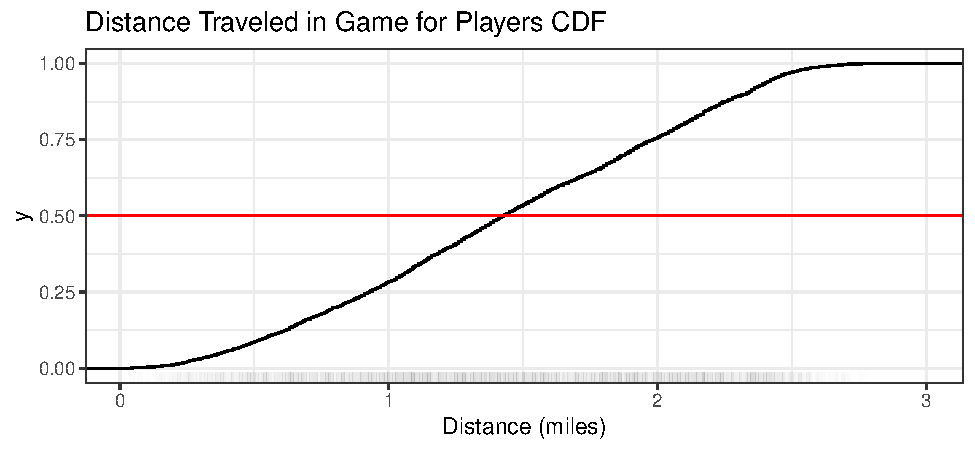
\includegraphics{EDA_files/figure-latex/unnamed-chunk-1-1.pdf}
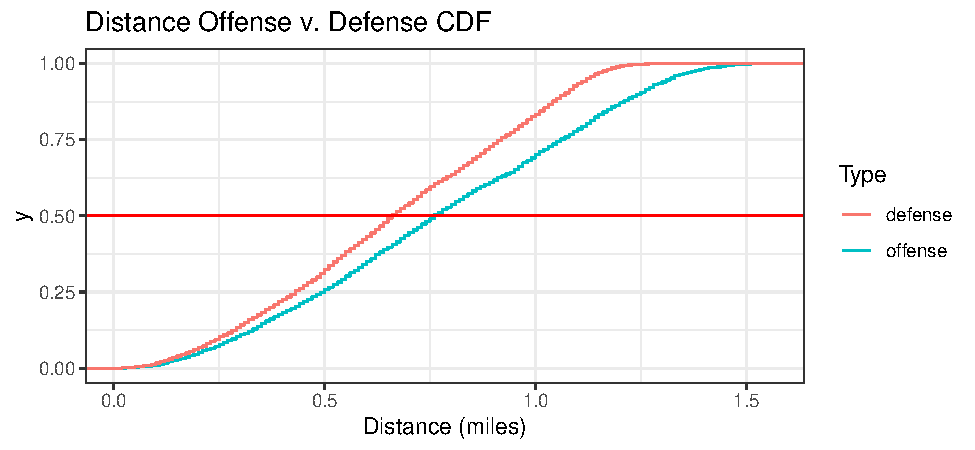
\includegraphics{EDA_files/figure-latex/unnamed-chunk-1-2.pdf}

\textbf{Entire Game:} min is 0.020, max is 2.990, and mean is 1.425
miles\\
\textbf{Offense:} min is 0.020, max is 1.560, and mean is .765 miles\\
\textbf{Defense:} min is .010, max is 1.29, and mean is .671 miles

\hypertarget{season-to-season}{%
\subsubsection{Season to Season}\label{season-to-season}}

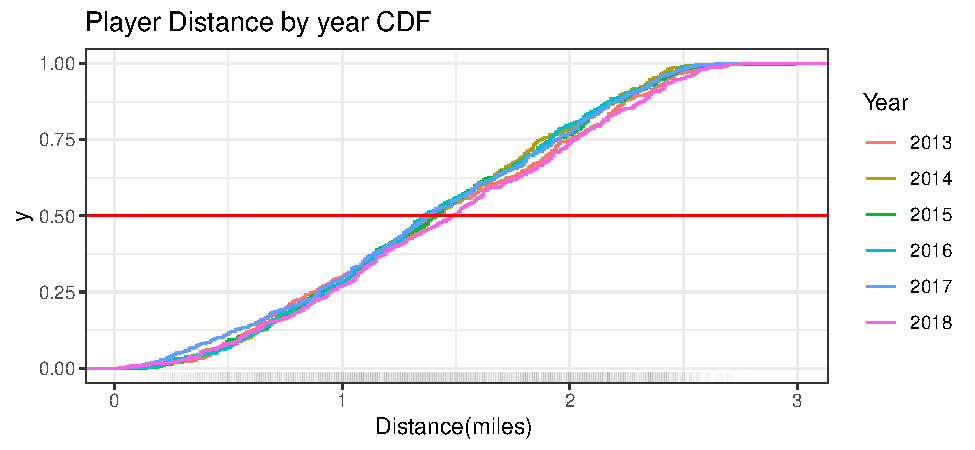
\includegraphics{EDA_files/figure-latex/unnamed-chunk-2-1.pdf}

\hypertarget{player-position}{%
\subsubsection{Player Position}\label{player-position}}

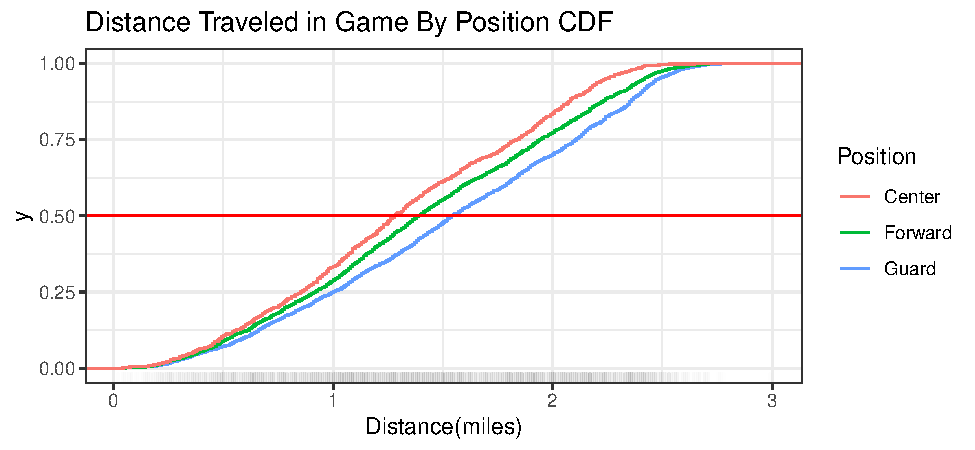
\includegraphics{EDA_files/figure-latex/unnamed-chunk-4-1.pdf}
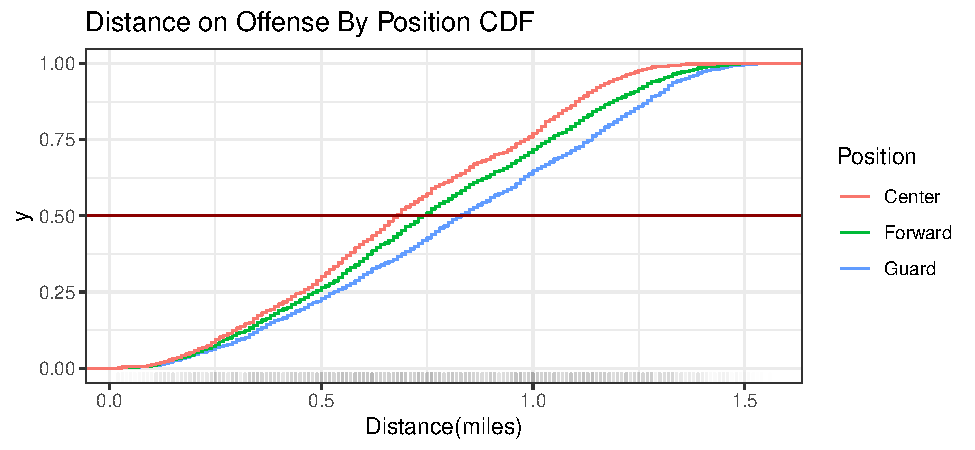
\includegraphics{EDA_files/figure-latex/unnamed-chunk-4-2.pdf}
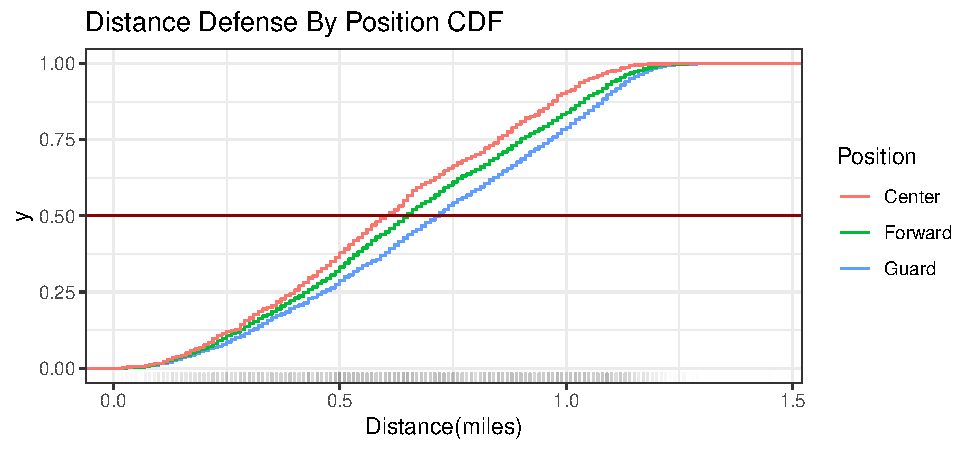
\includegraphics{EDA_files/figure-latex/unnamed-chunk-4-3.pdf}

\hypertarget{speed-in-game}{%
\subsubsection{Speed in Game}\label{speed-in-game}}

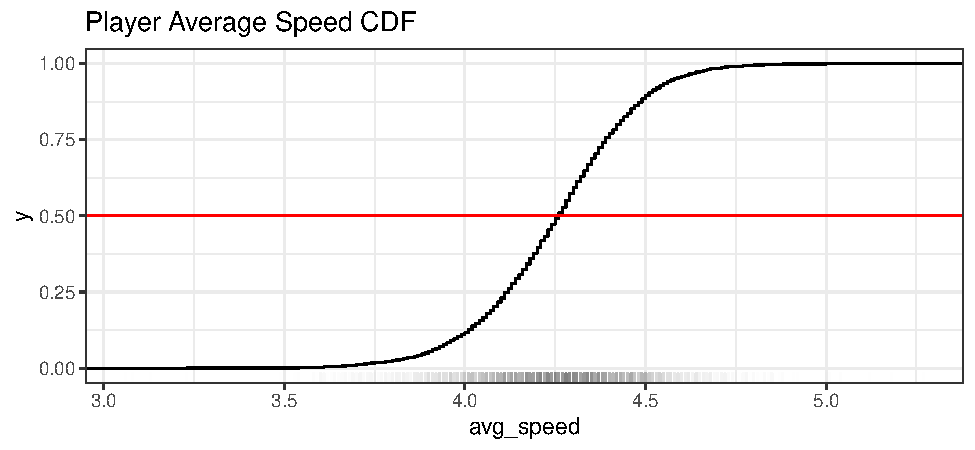
\includegraphics{EDA_files/figure-latex/unnamed-chunk-5-1.pdf}

\hypertarget{scatter-plots-looking-for-relationship-with-distance}{%
\subsubsection{Scatter plots looking for relationship with
distance}\label{scatter-plots-looking-for-relationship-with-distance}}

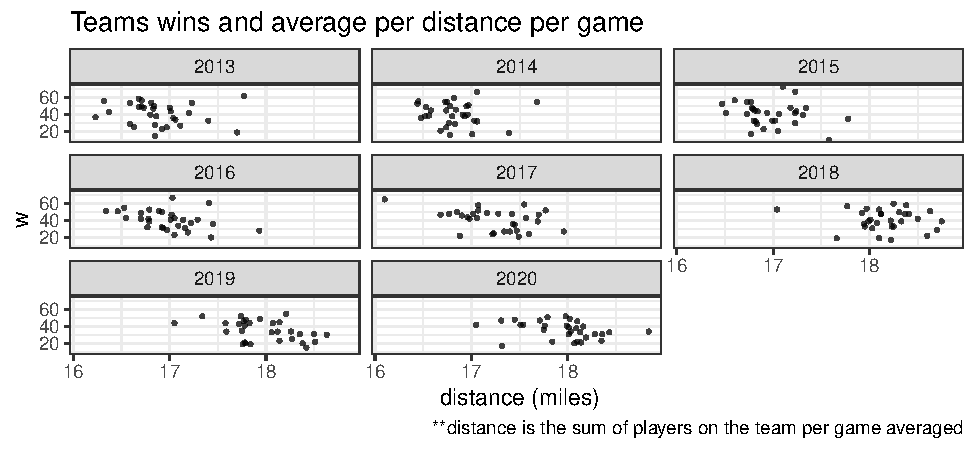
\includegraphics{EDA_files/figure-latex/unnamed-chunk-6-1.pdf}

\end{document}
